\documentclass[12pt]{article}
\usepackage[a4paper, bindingoffset=0.2in, %
							left=0.5in,right=0.5in,top=0.5in,bottom=0.5in,%
							footskip=.25in]{geometry}
\usepackage{graphicx}
\usepackage{amsmath}
\usepackage{physics}
\usepackage{hyperref}


\title{PSet6 Report}
\author{Ali Abolhassanzadeh Mahani}

\begin{document}
	\maketitle
	\section{Complex Networks}
	The Graphs and theirs degree and clustering distribution is shown in Fig\ref{fig:p1_1} for mean degree 0.8,
	Fig\ref{fig:p1_2} for mean degree 1.0 and Fig\ref{fig:p1_3} for mean degree 8.0.
	\begin{figure}[h!]
		\centering
		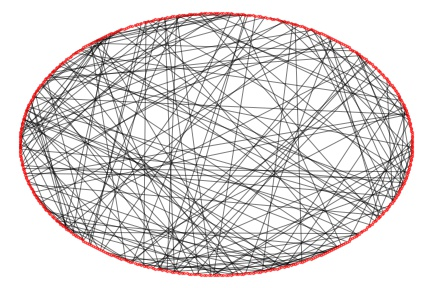
\includegraphics[width=0.4\linewidth]{../p1_0graph.jpg}
		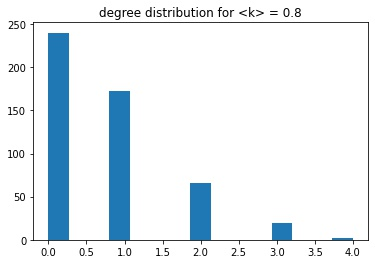
\includegraphics[width=0.4\linewidth]{../p1_0deg.jpg}
		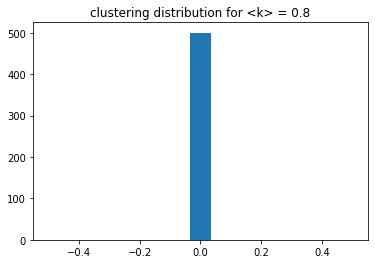
\includegraphics[width=0.4\linewidth]{../p1_0clust.jpg}
		\label{fig:p1_1}
		\caption{Illustrations for graph with mean degree of 0.8}
	\end{figure}

	\begin{figure}[h!]
	\centering
	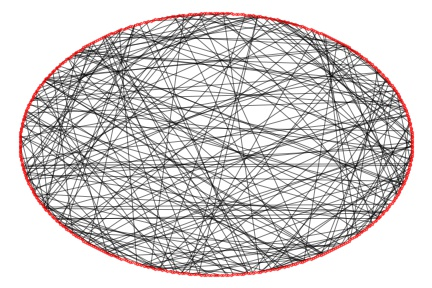
\includegraphics[width=0.4\linewidth]{../p1_1graph.jpg}
	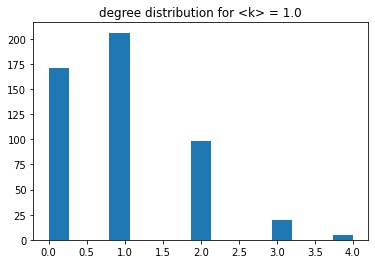
\includegraphics[width=0.4\linewidth]{../p1_1deg.jpg}
	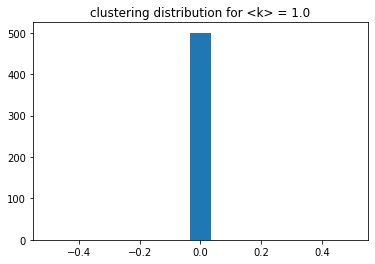
\includegraphics[width=0.4\linewidth]{../p1_1clust.jpg}
	\label{fig:p1_2}
	\caption{Illustrations for graph with mean degree of 1.0}
\end{figure}

	\begin{figure}[h!]
	\centering
	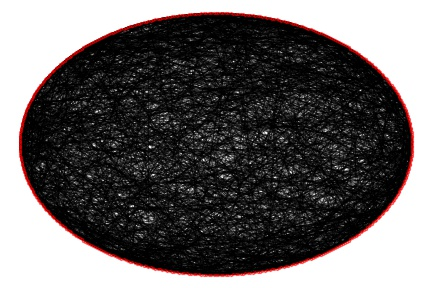
\includegraphics[width=0.4\linewidth]{../p1_8graph.jpg}
	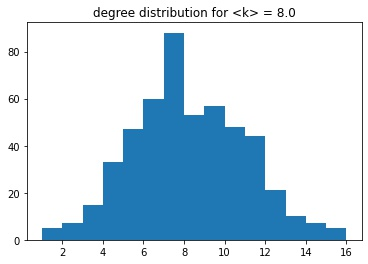
\includegraphics[width=0.4\linewidth]{../p1_8deg.jpg}
	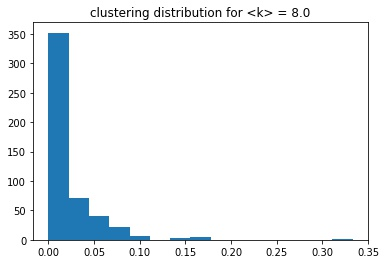
\includegraphics[width=0.4\linewidth]{../p1_8clust.jpg}
	\label{fig:p1_3}
	\caption{Illustrations for graph with mean degree of 8.0}
\end{figure}

	\section{Monte Carlo Integral(SS MC \& IS MC)}
	I did the SS MC and IS MC as wanted. I defined their functions and used \texttt{time.time()} to find the 
	runtime of the integration. The results are available in Table\ref{tab:MC}\\
	It's worth noting that the numeric value is roughly $0.8820814$. And for IS MC, the result of the integral of $g(x)$ is:\\
	\begin{equation}
		\int_0^2 e^{-x} = 1 - e^{-2}
	\end{equation}
	\begin{table}[h!]
		\centering
		\begin{tabular}{|c|c|c|c|c||c|c|c|c|}
			\hline
			n & \multicolumn{4}{|c||}{SS MC} & \multicolumn{4}{|c|}{IS MC} \\
			\hline
			n & I & $\Delta_{stat} I$ & $\Delta_{real} I$ & $t$ & I & $\Delta_{stat} I$ & $\Delta_{real} I$ & $t$ \\
			\hline
 			$1000$ & $0.858522$ & $0.546$ & $0.023$ & $0.02078$ & $0.882866$ & $0.0100$ & $0.00078$ & $0.01938$ \\
 			\hline
			 $2000$ & $0.861797$ & $0.55$ & $0.02$ & $0.01930$ & $0.871512$ & $0.007$ & $0.0106$ & $0.03906$ \\
			 \hline
			 $4000$ & $0.884244$ & $0.56$ & $0.0022$ & $0.05336$ & $0.875264$ & $0.005$ & $0.007$ & $0.08817$ \\
			 \hline
			 $8000$ & $0.886907$ & $0.56$ & $0.0048$ & $0.07861$ & $0.883804$ & $0.003$ & $0.002$ & $0.11154$ \\
			 \hline
			 $16000$ & $0.883410$ & $0.560$ & $0.0013$ & $0.14961$ & $0.882986$ & $0.002$ & $0.0009$ & $0.20379$ \\
			 \hline
			 $32000$ & $0.875776$ & $0.557$ & $0.0063$ & $0.19460$ & $0.881274$ & $0.0017$ & $0.0008$ & $0.39223$ \\
			 \hline
			 $64000$ & $0.879419$ & $0.558$ & $0.0027$ & $0.33243$ & $0.881791$ & $0.0012$ & $0.0003$ & $0.69962$ \\
			 \hline
		\end{tabular}
	\label{tab:MC}
	\caption{Data for numerical integration using SS MC and IS MC.}	
	\end{table}
	\section{The Sphere (Multi variable Integration SS MC)}
	Here the problem asks us to find the center of mass for the sphere with density
	$\rho(z) = \rho_0(1 - \frac{z}{4R})$ where $R$ is the radius of the sphere.\\
	This problem has a cylindrical symmetry. We take the sphere's bottom to lie on the origin
	and the center of the sphere on $z = R$ on the z-axis. This way the solution is as follows:
	\begin{equation}
		\begin{aligned} \label{eq:Analytic}
			MR_{CoM} = I &= \int_{0}^{2R} \rho(z) z \dd v = \int_{0}^{2R} \rho(z) z \pi \left(R^2 - (R - z)^2\right) 
			\dd z \\
			M &= \int_{0}^{2R} \dd m = \int_{0}^{2R} \rho(z) \pi \left(R^2 - (R - z)^2\right) \dd z\\
			\Rightarrow R_{CoM} &= \frac{I}{M}
		\end{aligned}
	\end{equation}
	
	We use IS MC with the function $\rho(z)$ as our distribution $g(z)$. This way we have:
	\begin{equation}
		\begin{aligned}
			I &= C \times \int_{0}^{2R} f(z) g(z) \dd z, \; C = \text{Const.},\\
			M &= C \times \int_{0}^{2R} h(z) g(z) \dd z,\\
			f(z) &= z \pi \left(R^2 - (R - z)^2\right),\\
			h(z) &= \pi \left(R^2 - (R - z)^2\right)\\
			\Rightarrow R_{CoM} &= \frac{\int_{0}^{2R} f(z) g(z) \dd z}{\int_{0}^{2R} h(z) g(z) \dd z}
		\end{aligned}
	\end{equation}
	using the equations in \ref{eq:Analytic}, we find:
	\begin{equation}
		\begin{aligned}
			I &= \frac{14}{15} \pi \rho_0 R^4,\\
			M &= \pi \rho_0 R^3\\
			\Rightarrow& R_{CoM} = \frac{14}{15} R
		\end{aligned}
	\end{equation}
	I made the random generator by finding the inverse of $g(z)$, took $\rho_0 = 1$ and
	$R = 10$, this leads to the numerical answer $R_{num} = 9.99854$ and the analytical result
	of $R_{real} =9.33333$ which raises the error to be about 
	$\delta = \frac{R_{num} - R_{real}}{R_{real}} \simeq 0.71 = 7.1 \%$
	
	\section{Metropolis Random Generation}
	 I made the function to generate random numbers with a normal distribution using the Metropolis Algorithm.\\
	 Then, I fount the steps in which the acceptance rate is $a.r. = \{0.9, 0.8, 0.7, 0.6, 0.5, 0.4, 0.3, 0.2, 0.1\}$\\
	 Then I made a function to find the correlation length (gyro length). There I used the fact that this length is equal to the first $j$ that gives an
	 auto-correlation of less than $e^{-1}$.
	 The result is in Table\ref{tab:rand}.
	 \begin{table}[h]
		\centering
		\begin{tabular}{|c|c|c|c|c|c|c|c|c|c|}
			\hline
			a. r. & $0.9$ & $0.8$ & $0.7$ & $0.6$ & $0.5$ & $0.4$ & $0.3$ & $0.2$ & $0.1$ \\
			\hline
			$\xi$ & $28$ & $9$ & $4$ & $3$ & $2$ & $2$ & $3$ & $4$ & $8$ \\
			\hline
		\end{tabular}
	\caption{The gyro length for each acceptance rate}
	\label{tab:rand}
	 \end{table}
	
	
\end{document}